%% abtex2-modelo-trabalho-academico.tex, v-1.9 laurocesar
%% Copyright 2012-2013 by abnTeX2 group at http://abntex2.googlecode.com/ 
%%
%% This work may be distributed and/or modified under the
%% conditions of the LaTeX Project Public License, either version 1.3
%% of this license or (at your option) any later version.
%% The latest version of this license is in
%%   http://www.latex-project.org/lppl.txt
%% and version 1.3 or later is part of all distributions of LaTeX
%% version 2005/12/01 or later.
%%
%% This work has the LPPL maintenance status `maintained'.
%% 
%% The Current Maintainer of this work is the abnTeX2 team, led
%% by Lauro César Araujo. Further information are available on 
%% http://abntex2.googlecode.com/
%%
%% This work consists of the files abntex2-modelo-trabalho-academico.tex,
%% abntex2-modelo-include-comandos and abntex2-modelo-references.bib
%%

% ------------------------------------------------------------------------
% ------------------------------------------------------------------------
% abnTeX2: Modelo de Trabalho Academico (tese de doutorado, dissertacao de
% mestrado e trabalhos monograficos em geral) em conformidade com 
% ABNT NBR 14724:2011: Informacao e documentacao - Trabalhos academicos -
% Apresentacao
% ------------------------------------------------------------------------
% ------------------------------------------------------------------------

\documentclass[
	% -- opções da classe memoir --
	12pt,				% tamanho da fonte
	openright,			% capítulos começam em pág ímpar (insere página vazia caso preciso)
	oneside,			% para impressão em verso e anverso. Oposto a oneside
	a4paper,			% tamanho do papel. 
	% -- opções da classe abntex2 --
	chapter=TITLE,		% títulos de capítulos convertidos em letras maiúsculas
	section=TITLE,		% títulos de seções convertidos em letras maiúsculas
	%subsection=TITLE,	% títulos de subseções convertidos em letras maiúsculas
	%subsubsection=TITLE,% títulos de subsubseções convertidos em letras maiúsculas
	% -- opções do pacote babel --
	english,			% idioma adicional para hifenização
	french,				% idioma adicional para hifenização
	spanish,			% idioma adicional para hifenização
	brazil				% o último idioma é o principal do documento
	]{abntex2}

% ---
% PACOTES
% ---

% ---
% Pacotes fundamentais 
% ---
%\usepackage{lmodern}			% Usa a fonte Latin Modern			
\usepackage{times}			% Usa a fonte Times
\usepackage[T1]{fontenc}		% Selecao de codigos de fonte.
\usepackage[utf8]{inputenc}		% Codificacao do documento (conversão automática dos acentos)
\usepackage{lastpage}			% Usado pela Ficha catalográfica
\usepackage{indentfirst}		% Indenta o primeiro parágrafo de cada seção.
\usepackage{color}			% Controle das cores
\usepackage{graphicx}			% Inclusão de gráficos
\usepackage{microtype} 			% para melhorias de justificação
\usepackage{listings}			% para inserir código fonte

% ---
% Pacotes de citações
% ---
\usepackage[brazilian,hyperpageref]{backref}	 % Paginas com as citações na bibl
\usepackage[alf]{abntex2cite}	% Citações padrão ABNT
\usepackage{titlesec}

% --- 
% CONFIGURAÇÕES DE PACOTES
% --- 

% altera o espacamento depois do número de cada secao, subsecao, etc
\titleformat{\section}
  {\normalfont\normalsize}{}{0pt}{\thesection\space}
\titleformat{\subsection}
  {\normalfont\normalsize\bfseries}{}{0pt}{\thesubsection\space}
\titleformat{\subsubsection}
  {\normalfont\normalsize}{}{0pt}{\thesubsubsection\space}
\titleformat{\paragraph}
  {\normalfont\normalsize\itshape}{}{0pt}{\theparagraph\space}

% ---
% Configurações do pacote backref
% Usado sem a opção hyperpageref de backref
\renewcommand{\backrefpagesname}{Citado na(s) página(s):~}
% Texto padrão antes do número das páginas
\renewcommand{\backref}{}
% Define os textos da citação
\renewcommand*{\backrefalt}[4]{
	\ifcase #1 %
		Nenhuma citação no texto.%
	\or
		Citado na página #2.%
	\else
		Citado #1 vezes nas páginas #2.%
	\fi}%
% ---

% ---
% **************************************************
% Informações que devem ser alteradas
% **************************************************
\titulo{\uppercase{ANÁLISE E DESENVOLVIMENTO DE UMA FERRAMENTA PARA AUTOMAÇÃO \\ DE CAPTAÇÃO DE ANÚNCIOS}}
\autor{\uppercase{Guilherme Santos}}
\orientador{Artur Todeschini Crestani}
\orientadortcc{Prof. \imprimirorientador, Esp. (SENAI/SC)}
\coordenador{Profa. Luciana Schimitz, Esp. (SENAI/SC)}
\coordenadortcc{Profa. Jaqueline Voltolini de Almeida, Me. (SENAI/SC)}
\examinador{Prof. Fulado de tal, Me. (SENAI/SC)}
\preambulo{Trabalho de Conclusão de Curso apresentado à Banca Examinadora do Curso Superior de Tecnologia em Análise e Desenvolvimento de Sistemas da Faculdade de Tecnologia do SENAI Florianópolis como requisito parcial para obtenção do Grau de Tecnólogo em Análise e Desenvolvimento de Sistemas.}
\proforientador{Professor Orientador: \imprimirorientador.}
\datadefesa{\uppercase{11 de dezembro de 2014}}
\local{Florianópolis/SC}
\data{2014}
% **************************************************

\instituicao{%
  SERVIÇO NACIONAL DE APRENDIZAGEM INDUSTRIAL 
  \par
  FACULDADE DE TECNOLOGIA SENAI/SC FLORIANÓPOLIS
  \par
  CURSO SUPERIOR DE TECNOLOGIA EM ANÁLISE E DESENVOLVIMENTO DE SISTEMAS}
%\tipotrabalho{Trabalho de Conclusão de Curso}

% alterando o aspecto da cor azul
\definecolor{blue}{RGB}{41,5,195}

% informações do PDF
\makeatletter
\hypersetup{
     	%pagebackref=true,
		pdftitle={\@title}, 
		pdfauthor={\@author},
    	pdfsubject={\imprimirpreambulo},
	    pdfcreator={LaTeX with abnTeX2},
		pdfkeywords={abnt}{latex}{abntex}{abntex2}{trabalho acadêmico}, 
		colorlinks=true,      	% false: boxed links; true: colored links
		linkcolor=black,	% color of internal links
		citecolor=black,        % color of links to bibliography
		filecolor=magenta,      % color of file links
		urlcolor=black,
		bookmarksdepth=4
}
\makeatother
% --- 

% --- 
% Espaçamentos entre linhas e parágrafos 
% --- 

% O tamanho do parágrafo é dado por:
\setlength{\parindent}{1.3cm}

% Controle do espaçamento entre um parágrafo e outro:
\setlength{\parskip}{0.2cm}  % tente também \onelineskip

%\titlespacing\section{0pt}{12pt plus 4pt minus 2pt}{-6pt plus 2pt minus 2pt}

% ---
% compila o indice
% ---
\makeindex
% ---

% ----
% Início do documento
% ----
\begin{document}

% Retira espaço extra obsoleto entre as frases.
\frenchspacing 

% ----------------------------------------------------------
% ELEMENTOS PRÉ-TEXTUAIS
% ----------------------------------------------------------

\imprimircapa
\imprimirfolhaderosto*

\begin{folhadeaprovacao}

  \begin{center}
    {\ABNTEXchapterfont\bfseries\normalsize\imprimirautor}

    \vspace*{\fill}\vspace*{\fill}
    \begin{center}
      \ABNTEXchapterfont\bfseries\normalsize\imprimirtitulo
    \end{center}
    \vspace*{\fill}
        \imprimirpreambulo
    \vspace*{\fill}
        
   APROVADA PELA {\bfseries{COMISSÃO EXAMINADORA}}
   \par
   EM FLORIANÓPOLIS, \bfseries{\imprimirdatadefesa}
   \end{center}

   \assinatura{\imprimircoordenador \\ Coordenador do Curso} 
   \assinatura{\imprimircoordenadortcc \\ Coordenador de TCC} 
   \assinatura{\imprimirorientadortcc \\ Orientador} 
   \assinatura{\imprimirexaminador \\ Examinador}
   \begin{center}
    \vspace*{1cm}
  \end{center}
\end{folhadeaprovacao}

% Arquivos que devem ser alterados
% ====================================================================
% Agradecimentos 
% ====================================================================
\begin{agradecimentos}
A Deus por possibilitar a conclusão de mais esta importante etapa em minha vida, por me fornecer força e determinação para não desistir durante o desenvolvimento deste trabalho.

Agradecimentos especiais à minha família que me apoiou psicologicamente e financeiramente durante todo o curso, que se não fosse o apoio que recebi, também não estaria concluindo este trabalho.

Agradeço ao SENAI e aos professores por todo o conhecimento repassado, que me ajudaram em minhas conquistas profissionais e pessoais e com certeza serão úteis para o resto da minha vida. Agradeço em especial ao meu orientador, Artur Todeschini Crestani, pelo conhecimento repassado, pelo apoio e tempo dedicado a me auxiliar durante este trabalho.
\end{agradecimentos}

% ====================================================================
% Epigrafe 
% ====================================================================
\begin{epigrafe}
    \vspace*{\fill}
	\begin{flushright}
		\textit{``A tarefa não é tanto ver aquilo que ninguém viu, mas pensar o que ninguém ainda pensou sobre aquilo que todo mundo vê''} \\
		(ARTHUR SCHOPENHAUER)
	\end{flushright}
\end{epigrafe}


% ====================================================================
% Resumo 
% ====================================================================

\noindent
SANTOS, Guilherme. \textbf{Análise e desenvolvimento de uma ferramenta para automação de captação de anúncios.}
Florianópolis, 2014. \pageref{nropaginas}f. Trabalho de Conclusão de Curso Superior de Tecnologia em
Análise e Desenvolvimento de Sistemas. Faculdade de Tecnologia do SENAI, Florianópolis, 2014.

\vspace{1cm}
\setlength{\absparsep}{18pt} % ajusta o espaçamento dos parágrafos do resumo
\begin{resumo}
 Segundo a NBR6028:2003, o resumo deve ressaltar o
 objetivo, o método, os resultados e as conclusões do documento. A ordem e a extensão
 destes itens dependem do tipo de resumo (informativo ou indicativo) e do
 tratamento que cada item recebe no documento original. O resumo deve ser
 precedido da referência do documento, com exceção do resumo inserido no
 próprio documento. (\ldots) As palavras-chave devem figurar logo abaixo do
 resumo, antecedidas da expressão Palavras-chave:, separadas entre si por
 ponto e finalizadas também por ponto.

 \textbf{Palavras-chave}: Latex. Abntex. Editoração de texto.
\end{resumo}

% ====================================================================
% Abstract 
% ====================================================================
\noindent
SANTOS, Guilherme. \textbf{Análise e desenvolvimento de uma ferramenta para automação de captação de anúncios.}
Florianópolis, 2014. \pageref{nropaginas}f. Trabalho de Conclusão de Curso Superior de Tecnologia em
Análise e Desenvolvimento de Sistemas. Faculdade de Tecnologia do SENAI, Florianópolis, 2014.

\vspace{1cm}
\begin{resumo}[\textbf{ABSTRACT}]
 \begin{otherlanguage*}{english}
   This is the english abstract.

   \vspace{\onelineskip}
 
   \noindent 
   \textbf{Key-words}: Latex. Abntex. Text editoration.
 \end{otherlanguage*}
\end{resumo}



% lista de figuras
\pdfbookmark[0]{\listfigurename}{lof}
\listoffigures*
\clearpage

% inserir lista de tabelas
\pdfbookmark[0]{\listtablename}{lot}
\listoftables*
\clearpage

% Arquivos que devem ser alterados
% ====================================================================
% Siglas 
% ====================================================================

\begin{siglas}
  \item[ANATEL] Agência Nacional de Telecomunicações.
  \item[APPS] Applications (em português, Aplicativos).
  \item[BITKOM] Associação Alemã de Tecnologia da Informação, Telecomunicações e Novas Mídias.
  \item[BPD] \textit{Business Process Diagram} (em português, Diagrama de Processos de Negócios).
  \item[BPM] \textit{Business Process Modeling} (em português, Modelagem de Processos de Negócio).
  \item[BPMI] \textit{Business Process Management Initiative} (em português, Iniciativa de Gestão de Processos de Negócio).
  \item[BPMN] \textit{Business Process Modeling Notation} (em português, Notação de Modelagem de Processos de Negócios).
  \item[DPN] Diagrama de Processos de Negócios.
  \item[IBOPE] Instituto Brasileiro de Opinião Pública e Estatística.
  \item[JVM] \textit{Java Virtual Machine} (em português, Máquina Virtual Java).
  \item[OHA] \textit{Open Handset Alliance}.
  \item[OMG] \textit{Object Management Group}.
  \item[OPEC] Operações Comerciais.
  \item[SEBRAE] Serviço Brasileiro de Apoio às Micro e Pequenas Empresas.
  \item[SENAI] Serviço Nacional de Aprendizagem Industrial.
  \item[TIC] Tecnologia da Informação e Comunicação.
  \item[UML] \textit{Unified Modeling Language} (em português, Linguagem de Modelagem Unificada).
   
\end{siglas}



% inserir o sumario
\pdfbookmark[0]{\contentsname}{toc}
\tableofcontents*
\clearpage

% ----------------------------------------------------------
% ELEMENTOS TEXTUAIS
% ----------------------------------------------------------
\textual

% PARTE - preparação da pesquisa
% ----------------------------------------------------------
%\part{Preparação da pesquisa}


% Informações que devem ser alteradas
% **************************************************
% ---
% Introdução
% ---
\chapter{INTRODUÇÃO}

O processo que envolve um anúncio de mídias impressas, como jornais, revistas e outros, passam por diversas etapas desde o cliente até a impressão final. Este processo não é muito conhecido e difundido, tanto na área de \textit{marketing} como na área da Tecnologia da Informação e Comunicação (TIC). Este trabalho tem como um de seus objetivos a compreensão, a análise e documentação com o uso de \textit{Business Process Modeling} (BPM) das etapas envolvidas no processo de anúncios. Com essa documentação referente ao processo, melhorias poderão ser fornecidas para aperfeiçoá-lo e também analisar onde um \textit{software} pode ser envolvido para realização de parte deste processo e por consequência a proposta do desenvolvimento de uma ferramenta que efetue uma das partes diagnosticadas no processo como que podem ser melhoradas. 

Este trabalho tem como objetivo fornecer um maior esclarecimento sobre o processo de anúncios e apresentar quais serão os resultados práticos e teóricos alcançados no final da análise e desenvolvimento do projeto.

Por meio da análise e desenvolvimento de um aplicativo móvel, que proporcione a captação do anúncio, seguindo a tendência do explosivo mercado de aplicativos móveis e o objetivo que estes aplicativos possuem, de fornecer cada vez mais mobilidade e autonomia para seus usuários. 

\begin{citacao}
O mercado de aplicativos para celulares cresce a cada ano, em todo o mundo são mais de 1,8 milhão de \textit{apps} disponíveis para os mais diversos tipos de usuários, além disso, o faturamento esperado para este ano deve alcançar a ordem de US\$ 29,5 bilhões. No Brasil, o mercado de celulares também está aquecido, segundo dados da Agência Nacional de Telecomunicações (Anatel) são mais de 265 milhões de linhas de celulares ativas no país \cite{sebrae2014}.
\end{citacao}

Com o uso do BPM, este trabalho pretende contribuir com a modelagem do processo de negócio existente e propor um novo clico de vida com os fluxos completamente redesenhados, tornando-o mais eficiente. A partir do processo existente modelado, é possível analisar e identificar os pontos desnecessários, duplicados e/ou que congestionam o processo. O processo e/ou os fluxos das atividades que são realizadas dentro dele, são redesenhados com a finalidade de propiciar uma maior agilidade, economia e o aumento do lucro em sua execução.

Apresenta-se uma visão sobre o mercado de dispositivos móveis e o desenvolvimento de aplicativos para os mesmos, com um estudo a respeito das principais tecnologias utilizadas para desenvolvimento nas principais plataformas móveis.


\section{JUSTIFICATIVA}

Segundo \citeonline[p. 178]{tanenbaum2003redes} os telefones celulares não são mais simples dispositivos eletrônicos que realizam chamadas e enviam mensagens de texto. Com o avanço da tecnologia, novos dispositivos como \textit{tablets} e \textit{smartphones}, que permitem o usuário acessar a \textit{internet} e a uma enorme variedade de aplicativos, surgiram e entraram no mercado de forma impactante. No Brasil o crescimento deste mercado mostra-se acompanhar os demais países do mundo. 

Em 2013, \citeonline[p. 64]{schuchTeletime} afirma que a Agência Nacional de Telecomunicações (ANATEL) divulgou uma estimativa sobre o número de dispositivos móveis no Brasil, esse número seria de 264 milhões (1,3 dispositivos por habitante), incluindo \textit{smartphones} e celulares convencionais, desse total, 68,2 milhões aparelhos possuem acesso à \textit{internet}.

Estudos também foram realizados pelo Instituto Brasileiro de Opinião Pública e Estatística (IBOPE) para comprovar o aumento do comércio e utilização de \textit{smartphones}. Segundo dados que o instituto recolheu das 42 maiores lojas online, em 2013 o \textit{e-commerce} brasileiro vendeu 1.841.880 \textit{smartphones}, que superou em 48\% a venda de celulares convencionais. O IBOPE identificou uma evolução expressiva do número de usuários de \textit{smartphones}, que de novembro de 2012 a junho de 2013 cresceu 25\%, chegando a quase 20 milhões de pessoas no país \cite{ibopeMobileEcommerce}.

O \citeonline{ibopeNovosProtagonistas, ibopeTablets} também realizou um levantamento sobre a venda de \textit{tablets} nas principais lojas de comércio eletrônico do Brasil. Os números apontam um total de 57 mil aparelhos vendidos no primeiro trimestre de 2012. No segundo trimestre de 2013, o crescimento das vendas chegou a 168\%, de abril a junho de 2013 foram vendidos 1,92 milhões de unidades, este aumento significativo pode ser explicado com a entrada no mercado de mais fabricantes destes dispositivos, causando a baixa do preço médio dos \textit{tablets}.

Segundo \citeonline[p. 12]{paivaTeletime}, a Flurry, empresa que analisa o mercado móvel, “acompanha o uso de 25 milhões de \textit{smartphones} no Brasil, este é o número de aparelhos que contam com pelo menos um aplicativo instalado com o código da empresa”. Os dispositivos móveis não mudaram apenas o mercado, mudaram também o cotidiano de seus usuários, que passaram a estar mais tempo acompanhando de seus aparelhos e possuir uma interação muito maior. 

\begin{citacao}
Quase 30\% dos mineiros e capixabas checam seus aparelhos assim que acordam e 61\% em situações de espera como em consultórios médicos, trânsito, transporte público ou cinema. Outras atividades em que eles utilizam seu aparelho foram levantadas, como no banheiro (21\%), durante as refeições (15\%) ou enquanto socializam (13\%). E, como última atividade do dia, 37\% estão com seus \textit{smartphones} antes de dormir, afirma o instituto \cite{ibopeNovosProtagonistas}.
\end{citacao}

Os usuários destes dispositivos passaram a realizar transações em seus aparelhos que antes eram realizadas pelo computador. Como transações bancárias, pagamentos de contas e também compras \textit{on-line}. 

Em uma pesquisa realizada com mineiros e capixabas, o \citeonline{ibopeNovosProtagonistas} informou que em maio de 2013 aproximadamente um terço deles gastou mais de 200 reais em compras realizadas pelo aparelho. Aplicativos e jogos para dispositivo móvel foram comprados por 39\% deles, eletrônicos por 34\% e compras coletivas por 33\%. 

Além disso, \citeonline[p. 20]{mouraFeMobilePayment} afirma que “no ano passado o PayPal registrou US\$ 14 bilhões em transações feitas por usuários por meio de dispositivos móveis (celulares, \textit{smartphones} e \textit{tablets}), contra US\$ 4 bilhões em 2011. Para este ano, a projeção da empresa é de atingir US\$ 20 bilhões”.

Em virtude do crescimento do mercado de dispositivos móveis, o mercado de aplicativos para estes dispositivos entrou em uma ascensão explosiva, \citeonline[p. 11]{paivaTeletime} afirma que "ao longo dos últimos cinco anos, a popularização de \textit{smartphones} gerou uma explosão de \textit{downloads} de \textit{apps}, o que atraiu mais desenvolvedores, inflando as lojas de aplicativos, agora com catálogos na casa de um milhão de títulos". \citeonline[p. 10]{paivaTeletime} ainda afirma que "existem cerca de 500 mil desenvolvedores de \textit{apps} móveis no mundo, desde amadores que têm atividade como um \textit{hobby} até empresas com faturamento anual na casa das centenas de milhões de dólares".


\section{OBJETIVOS}

Os objetivos da pesquisa são elencados a seguir.

\subsection{Objetivo geral}

Propor melhorias no processo de negócio de uma empresa de mídia impressa, a partir de análise e modelagem do modelo de negócio atual.

\subsection{Objetivos específicos}

\begin{enumerate}[label=\itshape\alph*\upshape)]
	\item Analisar e modelar o processo de negócio que foi analisado na empresa, utilizando a notação de modelagem de processos de negócios (BPMN).
	\item	Aperfeiçoar o processo de negócio que foi modelado com a BPMN, ou seja, a realização de um ciclo do BPM.
	\item	Propor e desenvolver um protótipo de um aplicativo móvel utilizando a plataforma Android, que contempla as atividades do processo em que é realizada a captação de anúncios pelos agentes e também possibilitará aos clientes do veículo publicar seus próprios anúncios sem necessitarem do intermédio de um funcionário da empresa. Não é o foco deste trabalho realizar a modelagem de engenharia de \textit{software} do aplicativo, será realizado apenas a modelagem e especificação de caso de uso para melhorar a compreensão do processo de negócio e das funcionalidades abordadas no protótipo a ser desenvolvido.
	
\end{enumerate}

% ---
% Capitulo de revisão de literatura
% ---
\chapter{REVISÃO DA LITERATURA}\label{cap-revisao}
Neste capítulo apresenta um estudo bibliográfico das tecnologias utilizadas para o desenvolvimento do trabalho.

\section{PROCESSOS DE NEGÓCIO}
Na construção de sua obra literária, \citeonline{baldamBPM} utiliza uma série de conceitos correlatos de diferentes fontes de referência para facilitar a compreensão de processos de negócios no seu contexto. Abaixo está transcrito o conceito de processos de negócios definido por Rozenfeld.

\begin{citacao}
É um fenômeno que ocorre dentro das empresas. Compreende um conjunto de atividades realizadas na empresa, associadas às informações que manipula, utilizando os recursos e a organização da empresa. Forma uma unidade coesa e deve ser focalizado em um tipo de negócio, que normalmente está direcionado a um determinado mercado/cliente, com fornecedores bem definidos \cite[p. 538]{rozenfeldProcesso}.
\end{citacao}

\subsection{Business Process Management (BPM)}
O \textit{Business Process Management} (BPM), segundo \citeonline{juniorMapeamentoGestaoProcessos}, pode ser definido como um conjunto de métodos, ferramentas e tecnologias que possuem objetivos em comum, como por exemplo: a) documentação do processo; b) efetuar treinamentos; c) estabelecimento de padrões de trabalho; d) respostas às mudanças; e) identificação de possíveis melhorias; f) desenho de um novo processo; g) comunicação; h) definição de novos requisitos; i) métricas de desempenho; j) automatização; k) permitir a simulação e análise de impacto; 

Os processos de negócios possuem níveis de hierarquia no BPM, para que tornar possível a representação de sua complexidade. São eles: a) processo, a abstração de mais alto nível; b) subprocesso, abstrações que possuem consolidação em níveis superiores e que também são decompostas em níveis inferiores; c) atividade, é o nível mais baixo da abstração, são processos que não possuem mais decomposição. Todos os elementos citados anteriormente são também são chamados de processos \cite{sordiGestaoModerna}.

Modelar um processo significa utilizar fluxos, diagramas ou mapas para representar graficamente a sequência de atividades que consolidam um processo. Esta representação deve chegar a um ponto de ser compreensível a todas as partes interessadas, desde o topo até a base da pirâmide organizacional. Para tornar esta tarefa possível, simples diagramas podem ser necessários para representar os pontos mais complexos do processo, seu nível de detalhamento e as ferramentas utilizadas dependem dos leitores do modelo \cite{juniorMapeamentoGestaoProcessos}.


\subsection{Business Process Modeling Notation (BPMN)}
No ano de 2004, o \textit{Business Process Management Initiative} (BPMI) publicou um padrão de notação chamado BPMN que havia sido desenvolvido por integrantes de algumas empresas como IBM, Pega, Lombardi, Ônix e iGrafx \cite{valleBarbaraBPMN}. No ano seguinte, o BPMI foi incorporado pela \textit{Object Management Group} (OMG), que se trata de uma associação aberta e sem fins lucrativos que é responsável pelo desenvolvimento de padrões utilizados na indústria de \textit{software} \cite{araujoGestao}.

\citeonline{valleBarbaraBPMN} definem a criação do BPMN como o produto final de um acordo entre empresas de ferramentas de modelagem que se reuniram com o intuito de criar uma linguagem para modelagem de processos de negócios, uma linguagem que fosse única e padronizada, facilitando assim o entendimento do usuário final. Os mesmos ainda ressaltam que o BPMN possui utilidade apenas como apoio a modelagem de conceitos aplicados a processos de negócios, ou seja, modelagens como a modelagem de estrutura organizacional e recursos, modelos de dados e informações e regras de negócios estão fora do escopo do BPMN. 

Para \citeonline{juniorMapeamentoGestaoProcessos}, o BPMN trata-se da maior, mais ampla e moderna notação para modelagem de processos que adotou um padrão de linguagem que resolve lacunas deixadas por métodos de modelagem anteriores, mesmo assim, ressaltam que a BPMN possui um ponto fraco significativo, por possuir uma linguagem particular, os elementos de notação não é difundida no grande público. 

É importante ressaltar, que mesmo \citeonline{valleBarbaraBPMN} definindo que o BPMN é utilizado para apoiar apenas a modelagem de processos de negócios, a notação de modelagem é aplicada em todos os ciclos de gestão por processos de negócios (BPM), tornando-se o principal responsável por integrar as pessoas interessadas com o processo \cite{sordiGestaoModerna}.

A finalidade de especificar processos de negócios é possuir uma documentação com qualidade, íntegro, não redundante e disponível para ser utilizado em toda a gestão de processo, permitindo seus usuários interagir com as operações do processo como monitorar e acompanhar seu desempenho por exemplo. Quando a BPMI desenvolveu a BPMN, seu principal objetivo era acabar com as perdas e dificuldades na interação entre o projeto lógico e físico. O BPMN foi criado para se tornar um padrão de comunicação entre todos os envolvidos (analistas de processos, técnicos, usuários, clientes e outros) com o processo de negócio, ele deve ser capaz de representar todos os complexos elementos dos processos de negócios atuais \cite{sordiGestaoModerna}.

Na especificação do processo de negócio pelo BPMN, são utilizados gráficos para representar de maneira simples, a lógica e os comportamentos mais complexos dos processos. Para que isso seja possível, é empregado um único diagrama, denominado de Diagrama de Processos de Negócios (DPN), ou \textit{Business Process Diagram} (BPD) \cite{araujoGestao}.

A figura \ref{fig-bpmn-exemplo} está exemplificado um simples diagrama DPN.
\\ \\ \\ \\ 

\begin{figure}[htb]
	\begin{center}
		\caption{
			\textbf{Diagrama de Processos de Negócios (DPN)}
		}\label{fig-bpmn-exemplo}
		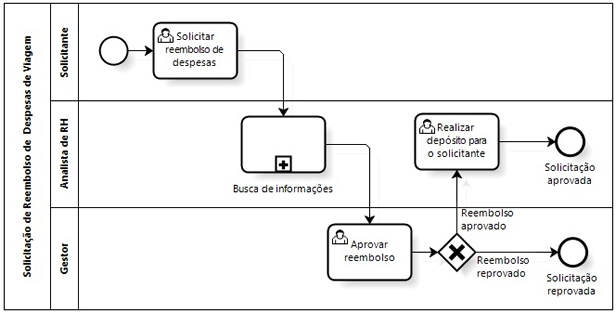
\includegraphics [scale=0.8]{imagens/bpmn_exemplo.jpg}
		\fonte{\citeonline{iprocessBpmn}}\label{fig-bpmn-exemplo}
	\end{center}
\end{figure}
 

\subsection{Processo}
Segundo \citeonline{baldamBPM} o processo aparece em várias situações para designar uma sequência de atividades: exemplo processos jurídicos, químicos. Neste trabalho o foco é o processo de negócios ou \textit{bussines process}, expressão que recupera o sentido do termo negócio, que não se restringe ao seu uso corrente no trato mercantil. 

A modelagem de processos de negócio envolve a descoberta, projeto e entrega de processo de negócios. Adicionalmente, o BPM inclui o controle executivo, administrativo e supervisório desses processos.

O propósito comum de todo o processo é transformar os recursos (entradas) em materiais de valor (saídas), como por exemplo, transformar materiais em aço ou informações em dados relevantes. Para tornar estas transformações possíveis, os processos necessitam de suprimentos, que são chamados de recursos de transformação, estes suprimentos podem ser colaboradores, equipamentos, \textit{softwares}, repositório de informações, entre outros \cite{baldamBPM}.

A figura \ref{fig-processo} ilustra como todos estes elementos (entradas, recursos de transformação e saídas) estão diretamente incluídos no processo.
\\

\begin{figure}[htb]
	\begin{center}
		\caption{
			\textbf{Visão sistêmica dos processos}
		}\label{fig-processo}
		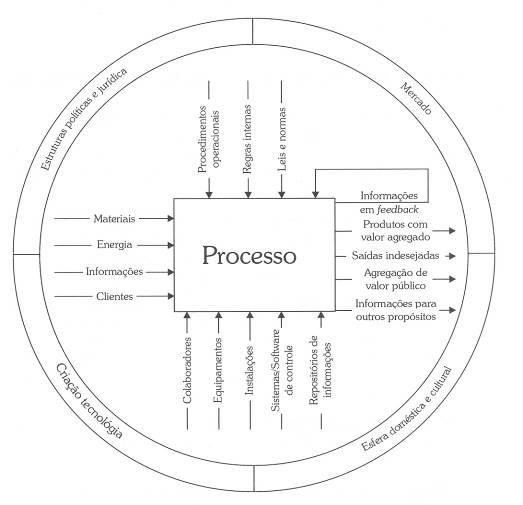
\includegraphics [scale=0.9]{imagens/processo.jpg}
		\fonte{\citeonline{baldamBPM}}\label{fig-processo}
	\end{center}
\end{figure}

Os autores \citeonline{erikssonPenkerUML} desenvolveram um conjunto de extensões baseadas em elementos de modelos da UML para representar elementos de um negócio. Estes elementos representam as entradas, recursos de transformação e saídas do processo, descritos anteriormente e ilustrados na figura \ref{fig-processo}. Com o diagrama do BPM é possível identificar o que é necessário para o processo acontecer (pré-condições), os envolvidos diretamente no processo (atores e outros elementos externos) e o seu resultado (pós-condição).

Na figura \ref{fig-macroprocesso} estão representados os elementos que são utilizados para representar um processo de negócio na UML.
\\ \\ \\

\begin{figure}[htb]
	\begin{center}
		\caption{
			\textbf{Elementos para representar o processo de negócio}
		}\label{fig-macroprocesso}
		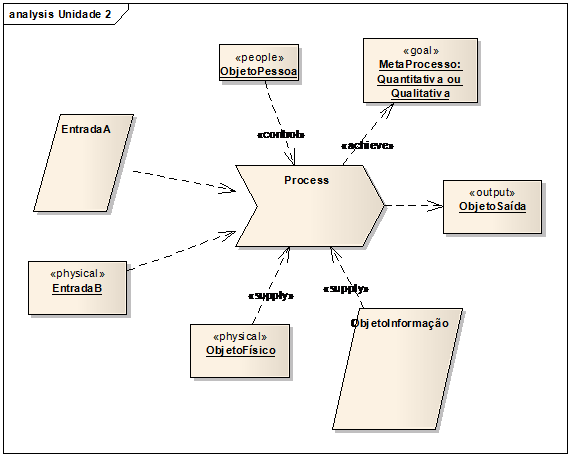
\includegraphics [scale=0.6]{imagens/macroprocesso.png}
		\fonte{\citeonline{erikssonPenkerUML}}\label{fig-macroprocesso}
	\end{center}
\end{figure}



\section{CASOS DE USO}
Caso de uso é uma descrição completa de um dos usos do sistema por um ator, ou seja, caso de uso é definido por \citeonline[p. 60]{bezerraUML} como a "especificação de uma sequência completa de interações entre um sistema e um ou mais agentes externos (atores)".

\begin{citacao}
Na terminologia da UML, qualquer elemento externo ao sistema que interage com o mesmo é, por definição, denominado ator. O termo "externo" nessa definição indica que atores não fazem parte do sistema. O termo "interage" significa que um ator troca informações com o sistema (envia informações para o sistema processar, ou recebe informações processadas provenientes do sistema). Atores representam a forma pela qual um sistema percebe seu ambiente. \cite[p. 60]{bezerraUML}.
\end{citacao}

Esta especificação tem como objetivo expor como ocorre o uso de uma funcionalidade do sistema, sem aprofundar-se na estrutura e detalhes internos do mesmo. A existência dessa característica revela que o modelo de caso de uso é um modelo com uma visão externa do sistema. O modelo de caso de uso permite visualizar quais são as funcionalidades e resultados providos pelo sistema.

Um caso de uso pode ser representado graficamente através de um diagrama, o diagrama de casos de uso. Este é um diagrama da \textit{Unified Modeling Language} (UML) que representa uma visão de alto nível do sistema. Atores, casos de uso e os seus relacionamentos são os elementos que compõem este diagrama e seu principal objetivo é mostrar como estes elementos inter-relacionam com as funcionalidades do sistema \cite{bezerraUML}. 
 

\section{PLATAFORMAS DE DESENVOLVIMENTO MÓVEL}
Ao estudar o assunto em relação ao desenvolvimento de aplicativos móveis, três tecnologias de desenvolvimento podem ser apontadas como as principais e consequentemente as mais encontradas nos aparelhos. Estas tecnologias são as plataformas Android da Google, iOS da Apple e Windows Phone da Microsoft.

\subsection{Android}
O Android é uma plataforma de desenvolvimento para aplicativos móveis, criada pelo grupo \textit{Open Handset Alliance} (OHA) e liderada pelo Google. O OHA foi criado com o objetivo de definir uma plataforma única e de código aberto para celulares, além de moderna e flexível para o desenvolvimento de aplicações corporativas. Como citado anteriormente, a licença da plataforma é livre (\textit{Apache Software Foundation}) permitindo assim que os fabricantes realizem alterações e customizem seus produtos, além de permitir que desenvolvedores criem aplicativos para seus próprios aparelhos. 

Segundo \citeonline[p. 23]{lechetaAndroid}, “o Android tem muitos diferenciais interessantes e uma arquitetura realmente flexível focada na integração de aplicações. Não existe diferença entre uma aplicação nativa e uma desenvolvida por você”. O sistema operacional utilizado na plataforma é o Linux, o mesmo é responsável pelo gerenciamento de memória, processos, \textit{threads}, redes, \textit{drivers} e a segurança arquivos e pastas. 

A linguagem de desenvolvimento utilizada no Android é o Java, porém os aplicativos não rodam na \textit{Java Virtual Machine} (JVM) e sim em outra máquina virtual chamada Dalvik, que foi aprimorada para executar em dispositivos móveis. 

A última versão disponibilizada da plataforma no desenvolvimento deste trabalho é o Android 4.4. O Google possui uma loja de aplicativos para a sua plataforma, a Google Play, anteriormente conhecida como Android Market.

\subsection{iOS}
O iOS é a plataforma de desenvolvimento móvel da Apple, inicialmente ele foi desenvolvido apenas para o iPhone, onde derivou seu nome, o iPhone OS, mas logo ele começou a ser utilizado em outros dispositivos como iPods, iPads e Apple TV, então passou a ser chamado apenas de iOS \cite{milaniIOS}. 

O sistema foi desenvolvido para ser executado apenas com os \textit{hardwares} também desenvolvidos pela empresa. Este é um dos diferenciais dos produtos da Apple, onde o \textit{software} consegue utilizar todos os recursos fornecidos pelo \textit{hardware}, atuando assim em conjunto. Outro diferencial da plataforma, é que seu sistema operacional possui uma interface elegante, simples e intuitiva \cite{milaniIOS}. 

A versão atual do iOS no desenvolvimento deste trabalho é a 8.1. Os aplicativos desenvolvidos para o iOS, geralmente são escritos com a linguagem de programação Objective-C, que também é utilizada no desenvolvimento para o sistema operacional Mac OS, mas também outras linguagens como C ou C++ podem ser utilizadas para o desenvolvimento dos aplicativos móveis. Um dos requisitos do desenvolvimento para iOS é um computador com o Mac OS. 

A Apple possui sua própria loja de aplicativos móveis para a sua plataforma, chamada App Store, onde desenvolvedores e empresas publicam seus aplicativos para a comunidade, cobrando algum preço ou até mesmo de graça \cite{pilonesIOS}.

\subsection{Windows Phone}
O Windows Phone é a plataforma de desenvolvimento de aplicativos móveis da Microsoft. A ideia da empresa é aumentar sua participação no mercado de dispositivos móveis, e entrou pesado na briga quando estabeleceu parcerias com outras grandes empresas do ramo da telefonia como Nokia, HTC e Samsung. 

A última versão lançada desta plataforma no desenvolvimento deste trabalho é a Windows Phone 8 que “se destaca como uma das principais plataformas de desenvolvimento \textit{mobile} do mercado e possui uma interface única e muito focada na experiência do usuário”, afirma \citeonline[p. 16]{lechetaWindows}. 

A linguagem de programação utilizada para desenvolvimento nesta plataforma é a C\#, também criada pela Microsoft, além deste requisito para o desenvolvimento de aplicativos, outra restrição é que o mesmo seja realizado em um ambiente com o sistema operacional Windows 8. 

Assim como as outras plataformas citadas nos parágrafos anteriores, a Microsoft também possui a sua loja de aplicativos para a plataforma, a Windows Phone Store.


\section{WEBSERVICE}

\subsection{REST}


% ---
% Procedimentos metodológicos
% ---
\chapter{PROCEDIMENTOS METODOLÓGICOS}

Segundo \citeonline[p. 1]{gilPesquisa}, a pesquisa é definida como o "procedimento racional e sistemático que tem como objetivo proporcionar respostas aos problemas que são propostos". Ele ainda afirma que a pesquisa é necessária quando não existe informação suficiente para o problema, ou "então quando a informação disponível se encontra em tal estado de desordem que não possa ser adequadamente relacionada ao problema” \cite[p. 1]{gilPesquisa}. No presente trabalho fez-se o uso da pesquisa exploratória, da estratégia de pesquisa bibliográfica e da avaliação qualitativa.

Por se tratar de um tema interdisciplinar e os conteúdos sobre ele serem escassos, a pesquisa assumiu um caráter exploratório, com o objetivo de prover maior intimidade ao problema e ao tema, com o intuito de torná-los mais transparentes e compreensíveis. As técnicas de coletas de dados e informações geralmente utilizadas são as de “levantamento bibliográfico e de entrevistas com pessoas que tiveram experiência prática com o assunto” \cite[p. 27]{gilPesquisa} e foram as utilizadas pelo autor.

A pesquisa bibliográfica é definida por ser uma “estratégia de pesquisa necessária para a condução de qualquer pesquisa científica. Uma pesquisa bibliográfica procura explicar e discutir um assunto, tema ou problema” \cite[p. 54]{martinsTheophiloMetodologia}. Esta estratégia utiliza de conteúdos publicados em livros, periódicos, revistas, jornais, enciclopédias, dicionários, teses, dissertações, anais de eventos científicos e sites.

Para o conhecimento teórico referente às principais tecnologias das plataformas de desenvolvimento móvel, o crescimento do mercado de dispositivos móveis e consequentemente o crescimento do mercado de desenvolvimento para estes dispositivos e também sobre o BPM foram adquiridos por meio de levantamento bibliográfico em livros, revistas e monografias, encontrados na biblioteca do SENAI Florianópolis e também em sites de instituições educacionais e de pesquisa e estatística.

As técnicas adotadas para a coleta de dados, informações e evidências utilizadas pelo autor foram as de levantamento bibliográfico e de entrevistas. Estas técnicas são importantes para a pesquisa, pois permitem o autor analisar as informações necessárias referentes ao tema e realizar o desenvolvimento e as conclusões de sua pesquisa.

Os dados obtidos no levantamento bibliográfico foram dados secundários, que segundo \citeonline[p. 85]{martinsTheophiloMetodologia} são os dados “já coletados que se encontram organizados em livros, banco de dados, anuários estatísticos, relatórios, etc”. Através de revistas e sites, foram levantados os dados referentes ao crescimento dos mercados de dispositivos móveis e aplicativos móveis.

As entrevistas são definidas pelos autores \citeonline[p. 88]{martinsTheophiloMetodologia} como “uma técnica de pesquisa para coleta de informações, dados e evidências cujo objetivo básico é entender e compreender o significado que entrevistados atribuem a questões e situações em contextos que não foram estruturados anteriormente”. Foram realizadas entrevistas semi estruturadas, que é conduzida sem um roteiro, mas podendo o entrevistador acrescentar novas questões, com o sócio e diretor técnico de uma empresa privada, que trabalha há 20 anos com mídias impressas. As entrevistas tinham como objetivo a compreensão e o esclarecimento sobre o processo de um anúncio, desde sua captação até a publicação.

A pesquisa qualitativa tem como preocupação central descrições, compreensões e interpretações dos fatos ao invés de medições, afirmam \citeonline[p. 141]{martinsTheophiloMetodologia}. Justifica-se a abordagem qualitativa quando existe pouca informação a respeito do assunto a ser pesquisado, sendo necessários explorar o conhecimento que as pessoas possuem com base em suas experiências. Os dados qualitativos levantados com a pesquisa foram as citações diretas de pessoas sobre suas experiências, referente ao processo de um anúncio. Estes dados foram captados através da técnica de entrevista.


% ---
% Resultados
% ---
\chapter{RESULTADOS E DISCUSSÕES}


\section{PROCESSO ATUAL}
O processo que envolve a captação de anúncio de veículos de mídias impressas foi levantado e projetado pelo autor através de entrevistas (informação verbal)\footnote{Informação fornecida pelo diretor de desenvolvimento de uma empresa de desenvolvimento de \textit{softwares} em Florianópolis, em Abril de 2014.} e por sua experiência trabalhando em uma empresa de desenvolvimento de \textit{softwares} para veículos de comunicação.

Visando documentar o processo levantado pelo autor, foi modelado um diagrama de macroprocesso para representar o modelo atual do processo. A figura \ref{fig-diag-macroprocesso} apresenta a ilustração do macroprocesso.

\begin{figure}[h]
	\begin{center}
		\caption{
			\textbf{Diagrama de macroprocesso do processo atual}
		}\label{fig-diag-macroprocesso}
		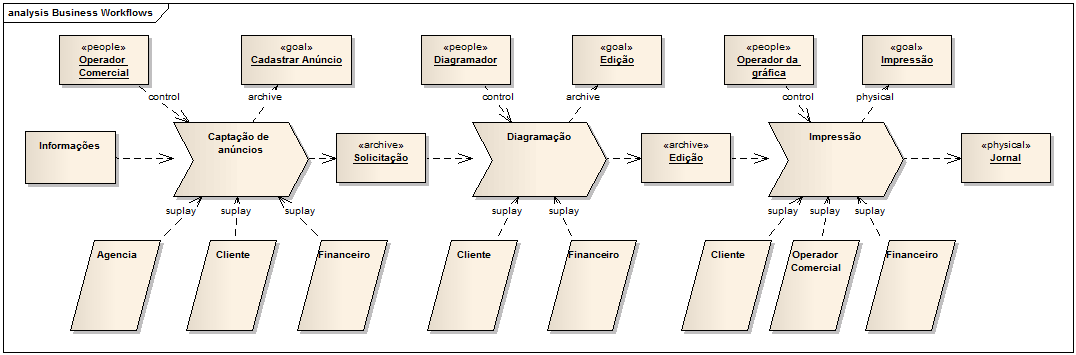
\includegraphics [scale=0.58]{imagens/diagrama_macro_processo.png}
		\fonte{AUTOR (2014)}\label{fig-diag-macroprocesso}
	\end{center}
\end{figure}


A captação e o cadastro de anúncios para os veículos de mídia impressa é realizada por um departamento chamado de Operações Comerciais (OPEC). Os anúncios chegam até a OPEC pelo contato direto com o cliente ou pelo intermédio de agentes de vendas, do próprio veículo ou de agências de publicidade. A OPEC recebe os pedidos de anúncios e os insere na base de dados.

Outra responsabilidade deste departamento é receber as artes (imagens) dos anúncios que utilizam alguma espécie de personalização, estas podem ser produzidas pelo próprio cliente ou por uma agência de propaganda. Quando o cliente não possuir uma arte, a mesma pode ser desenvolvida no departamento de arte do veículo, cabe a OPEC solicitar a sua produção.

Gerada a cobrança do anúncio pelo departamento financeiro e com sua arte pronta caso possuir, cabe ao departamento de diagramação inserir o anúncio juntamente com os outros itens do produto nas edições a serem impressas. Após a impressão do produto (jornal, revista, folheto, entre outros), a situação do anúncio é atualizada informando sua impressão.

A figura \ref{fig-bpmn-processo-atual} apresenta a modelagem do processo otimizado utilizando a notação BPMN. A partir deste modelo, é possível visualizar detalhadamente cada fluxo do processo atual.

\begin{figure}[h]
	\begin{center}
		\caption{
			\textbf{Diagrama de BPMN do processo atual}
		}\label{fig-bpmn-processo-atual}
		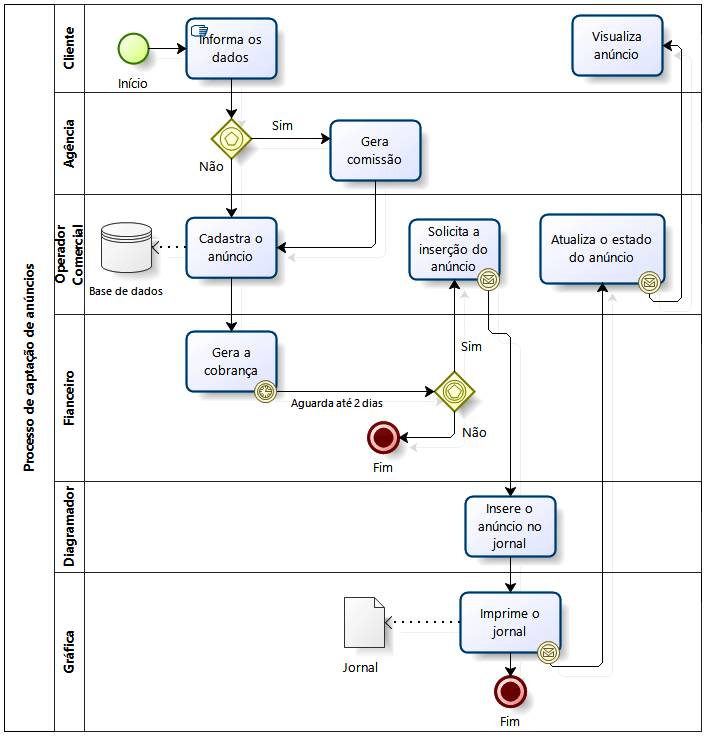
\includegraphics [scale=0.84]{imagens/bpmn_processo_atual.png}
		\fonte{AUTOR (2014)}\label{fig-bpmn-processo-atual}
	\end{center}
\end{figure}


\section{OTIMIZAÇÃO DO PROCESSO}

A análise do processo de negócios possibilitou o levantamento e a identificação dos requisitos necessários para o processo e dos requisitos que poderiam ser abolidos do mesmo, tornando assim o processo mais eficiente.

A partir da figura \ref{fig-diag-macroprocesso}, é possível analisar que a OPEC e o diagramador são papéis que podem ser removidos do processo, onde o cliente teria autonomia para enviar seu próprio anúncio a ser impresso, não necessitando do intermédio de funcionários do veículo.

A figura \ref{fig-diag-macroprocesso-otimizado} apresenta o modelo proposto do macroprocesso otimizado pelo autor.
\begin{figure}[h]
	\begin{center}
		\caption{
			\textbf{Diagrama de macroprocesso do processo otimizado}
		}\label{fig-diag-macroprocesso-otimizado}
		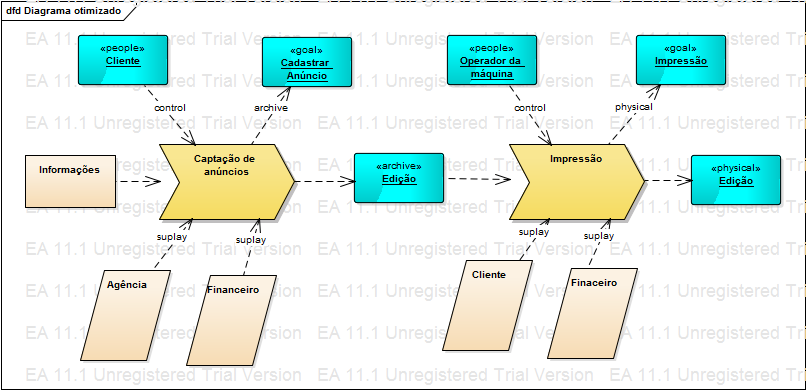
\includegraphics [scale=0.65]{imagens/diagrama_macro_processo_otimizado.png}
		\fonte{AUTOR (2014)}\label{fig-diag-macroprocesso-otimizado}
	\end{center}
\end{figure}

Para contemplar este modelo, é necessário o uso do aplicativo móvel para captação de anúncios que também foi proposto pelo autor. Através do aplicativo, o cliente ou até mesmo os agentes de captação de anúncios, podem inserir imediatamente o anúncio na base de dados do veículo, sem necessitar da participação da OPEC.

Com a cobrança e a inserção dos anúncios também automatizados, o envio do anúncio cadastrado pelo aplicativo será direto para a impressão, reduzindo o número de etapas e recursos necessários para o processo poder ser realizado.

A figura \ref{fig-bpmn-processo-otimizado} apresenta a modelagem do processo otimizado utilizando a notação BPMN. Analisando este modelo, é possível notar que o número de fluxos diminuiu, pois os passos que passavam pela agência, operador comercial e pelo Diagramador não estão mais presentes ou foram realocados. 

\begin{figure}[h]
	\begin{center}
		\caption{
			\textbf{Diagrama de BPMN do processo otimizado}
		}\label{fig-bpmn-processo-otimizado}
		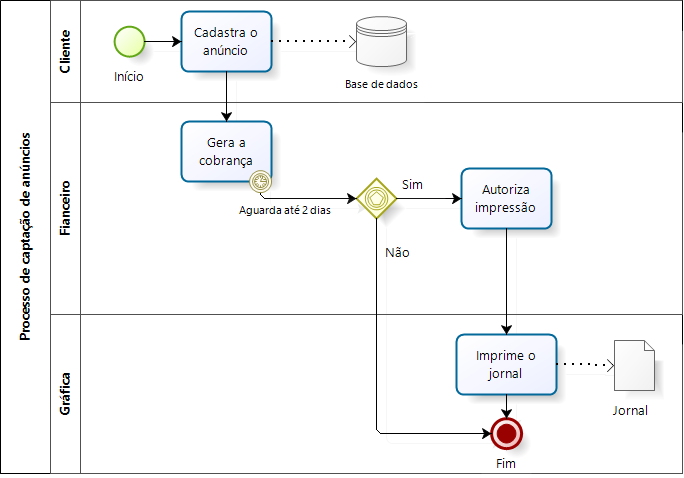
\includegraphics [scale=0.84]{imagens/bpmn_processo_otimizado.png}
		\fonte{AUTOR (2014)}\label{fig-bpmn-processo-otimizado}
	\end{center}
\end{figure}

\section{MODELO DE CASO DE USO}
Com a modelagem do processo de negócio, foi possível identificar os atores envolvidos com o processo. A partir deste resultado, a modelagem de caso de uso foi desenvolvida para definir as interações dos atores com o sistema e outros elementos externos.

A figura \ref{fig-modelo-uc} apresenta o diagrama de caso de uso, possibilitando visualizar os requisitos levantados pelo autor no desenvolvimento do trabalho. \\ \\ \\ \\ \\ \\ \\ \\ \\ \\

\begin{figure}[h]
	\begin{center}
		\caption{
			\textbf{Modelo de Caso de Uso}
		}\label{fig-modelo-uc}
		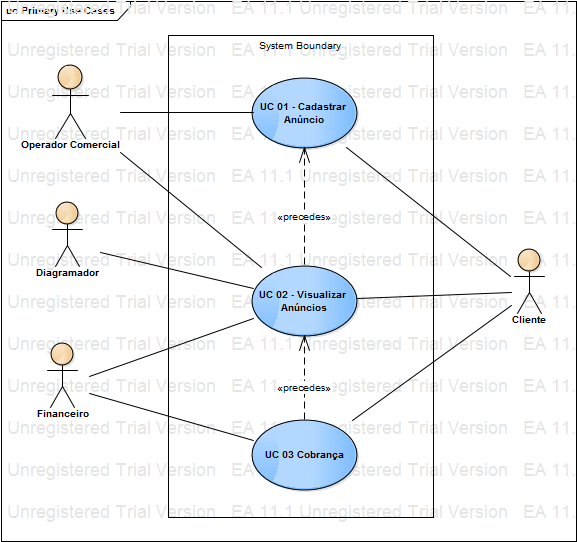
\includegraphics [scale=0.6]{imagens/modelo_caso_de_uso.png}
		\fonte{AUTOR (2014)}\label{fig-modelo-uc}
	\end{center}
\end{figure}

As tabelas \ref{tab-csu-cadastrarAnuncio} e \ref{tab-csu-visualizarAnuncios} estão detalhados apenas os casos de uso que foram contemplados pelo autor no desenvolvimento do aplicativo móvel. \\ \\ \\ \\ \\ \\ \\ \\ \\ \\ \\ \\ \\ \\ \\

\begin{table}[Htp!]
	\begin{center}
		\def\arraystretch{1.5}
		\caption{\textbf{Caso de uso: Cadastrar Anúncio}}
		\label{tab-csu-cadastrarAnuncio}
		\begin{tabular}{|l|}
			\hline
			\multicolumn{1}{|c|}{\textbf{Cadastrar Anúncio (CSU01)}} \\ \hline
			
			
			\textbf{Sumário:} O ator usa o sistema para cadastrar um anúncio de classificados \\de jornal impresso. \\
			\textbf{Ator Primário:} Cliente. \\
			\textbf{Precondições:} O ator deve estar autenticado no sistema. \\ \hline
			
			\textbf{Fluxo Principal:} O caso de uso se inicia quando o ator acessa o sistema\\ e seleciona a opção "Novo anúncio". \\
			
			
			1.	O sistema solicita ao ator as informações de cadastro do anúncio. \\
			2.	O ator preenche com as informações necessárias. \\
			3.  O ator seleciona a opção "Salvar". \\
			4.  O sistema valida as informações. \\
			5.  O sistema retorna uma mensagem confirmando o cadastro. \\
			6.	O caso de uso é encerrado. \\ \hline
			
			\textbf{Fluxo Alternativo (3):} Cancelar.\\ 
			a. O ator solicita o cancelamento da execução do passo 3 do fluxo básico.\\
			b. O sistema encerra o cadastro. \\
			c. O caso de uso é encerrado. \\ \hline
			
			\textbf{Fluxo de Exceção (4):} Dados inválidos.\\
			a. O ator informou dados que não satisfaçam as validações do sistema, \\então o sistema retorna ao passo 1 informando qual validação não foi\\ satisfeita.\\ \hline
			
			\textbf{Pós-condições:} Deve-se manter a integridade dos dados sobre um\\ anúncio e seus relacionamentos. \\ \hline
			
		\end{tabular}
		\fonte{AUTOR (2014)}
	\end{center}
\end{table}


\begin{table}[Htp!]
	\begin{center}
		\def\arraystretch{1.5}
		\caption{\textbf{Caso de uso: Visualizar Anúncios}}
		\label{tab-csu-visualizarAnuncios}
		\begin{tabular}{|l|}
			\hline
			\multicolumn{1}{|c|}{	\textbf{Visualizar Anúncios (CSU02)}} \\ \hline
			
			
			\textbf{Sumário:} O ator visualiza seus últimos anúncios cadastrados no sistema. \\
			\textbf{Ator Primário:} Cliente. \\
			\textbf{Precondições:} O ator deve estar autenticado no sistema. \\ \hline
			
			
			\textbf{Fluxo Principal:} O Caso de uso se inicia quando o ator acessa o sistema e \\ entra em sua página inicial ou seleciona a opção "Meus anúncios". \\
			
			
			1.	O sistema exibe os últimos anúncios cadastrados pelo autor. \\
			2.	O ator visualiza seus últimos anúncios cadastrados. \\
			3.	O caso de uso é encerrado. \\ \hline


			\textbf{Fluxo de Exceção (2):} Nenhum anúncio cadastrado. \\
			a. O ator ainda não cadastrou nenhum anúncio, o sistema informa o fato e o \\ caso de uso é encerrado. \\ \hline
			
			\textbf{Pós-condições:} O ator visualiza seus últimos anúncios cadastrados. \\ \hline

		\end{tabular}
		\fonte{AUTOR (2014)}
	\end{center}
\end{table}



\section{APLICAÇÃO}

Foi desenvolvido um protótipo de um aplicativo móvel para a plataforma Android que permite o seu usuário a salvar e visualizar seus anúncios já cadastrados. Também foi desenvolvido um protótipo de uma aplicação \textit{web} que é possível visualizar todos os anúncios salvos na base de dados. A figura \ref{fig-estrutura-aplicacoes} apresenta a estrutura dos protótipos desenvolvidos. \\ \\ \\ \\ \\ \\ \\ \\ \\ \\ \\ \\ \\

\begin{figure}[h]
	\begin{center}
		\caption{
			\textbf{Estrutura das aplicações desenvolvidas}
		}\label{fig-estrutura-aplicacoes}
		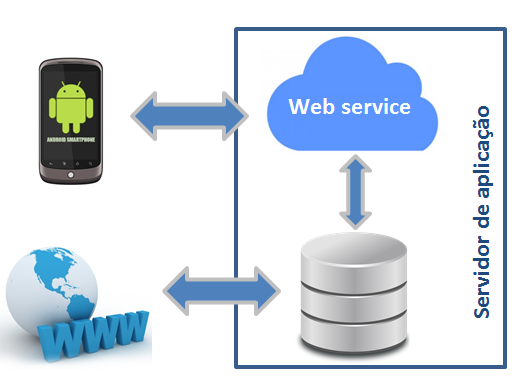
\includegraphics [scale=0.7]{imagens/arquitetura.png}
		\fonte{AUTOR (2014)}\label{fig-estrutura-aplicacoes}
	\end{center}
\end{figure}

O aplicativo Android comunica-se com o servidor de aplicação por meio de um \textit{webservice} REST para acessar os anúncios do usuários e inserir novos no banco de dados. Já a aplicação \textit{web} não utiliza \textit{webservice} para se comunicar com o servidor de aplicação, pois ela está instalada no mesmo servidor e pode comunicar-se diretamente com o banco de dados. Através da aplicação \textit{web} é possível visualizar os anúncios de todos os usuários da base de dados, além da listagem, é possível visualizar detalhadamente cada anúncio. 

\subsection{Aplicativo Android}

Um dos objetivos do trabalho era o desenvolvimento de um protótipo de um aplicativo Android que contemplasse o modelo otimizado do processo de negócio da captação de anúncio. Através do aplicativo, o cliente tem liberdade de inserir seu próprio anúncio e visualizar seus anúncios já enviados. As figuras a seguir apresentam as telas e funcionalidades desenvolvidas no protótipo.

A figura \ref{fig-android-login} mostra a tela inicial do aplicativo, é nesta tela que o usuário autentica-se. Ao clicar no botão "Entrar", o aplicativo leva o usuário até a tela "Home" com seus anúncios já cadastrados. \\ \\ \\ \\ \\

\begin{figure}[h]
	\begin{center}
		\caption{
			\textbf{Tela inicial do aplicativo}
		}\label{fig-android-login}
		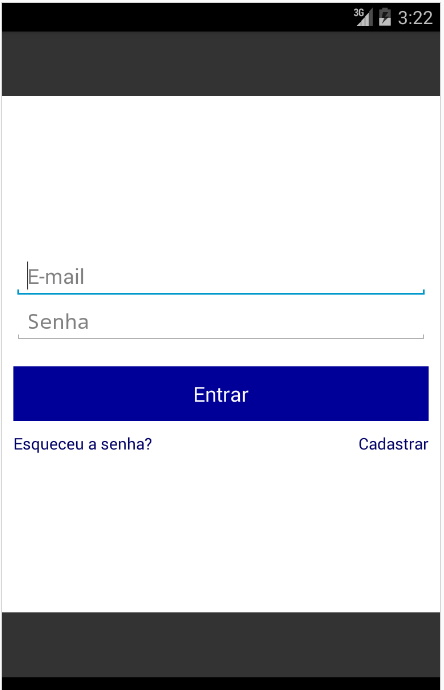
\includegraphics [scale=0.6]{imagens/android-login.png}
		\fonte{AUTOR (2014)}\label{fig-android-login}
	\end{center}
\end{figure}


A figura \ref{fig-android-meus-anuncios} apresenta a tela seguinte a autenticação do usuário. Ela possui um botão para ir para o menu, o nome do veículo que o aplicativo foi desenvolvido, o nome do usuário que esta utilizando o aplicativo e os seus anúncios cadastrados em ordem decrescente. Ao clicar no botão "Menu" ele leva usuário até a tela de menu do aplicativo. \\ \\ \\ \\ \\ \\ \\ \\ \\ \\ \\ \\ \\

\begin{figure}[h]
	\begin{center}
		\caption{
			\textbf{Tela de visualização dos anúncios cadastrados}
		}\label{fig-android-meus-anuncios}
		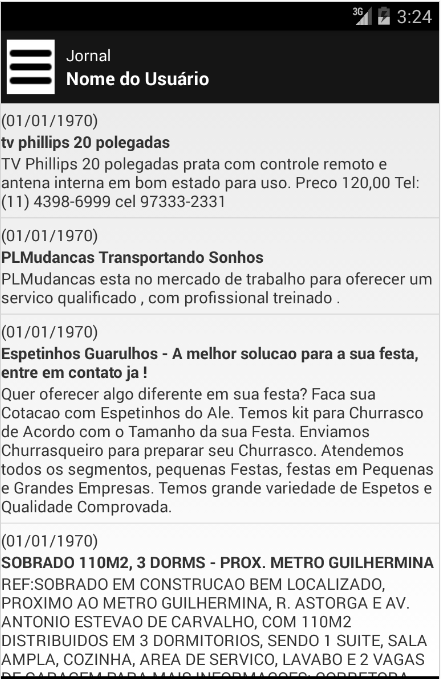
\includegraphics [scale=0.6]{imagens/android-meus-anuncios.png}
		\fonte{AUTOR (2014)}\label{fig-android-meus-anuncios}
	\end{center}
\end{figure}

A figura \ref{fig-android-menu} apresenta tela de menu do aplicativo, ela possui o nome do veículo que o aplicativo foi desenvolvido, o nome do usuário que esta utilizando o aplicativo e as opções do menu: a) "Home", leva o usuário até a tela de visualização dos anúncios cadastrados; b) "Novo anúncio", leva o usuário a tela de cadastro de um novo anúncio; c) "Sair", fecha o aplicativo. \\ \\ \\ \\ \\ \\ \\ \\ \\ \\ \\ \\ \\

\begin{figure}[h]
	\begin{center}
		\caption{
			\textbf{Tela de menu}
		}\label{fig-android-menu}
		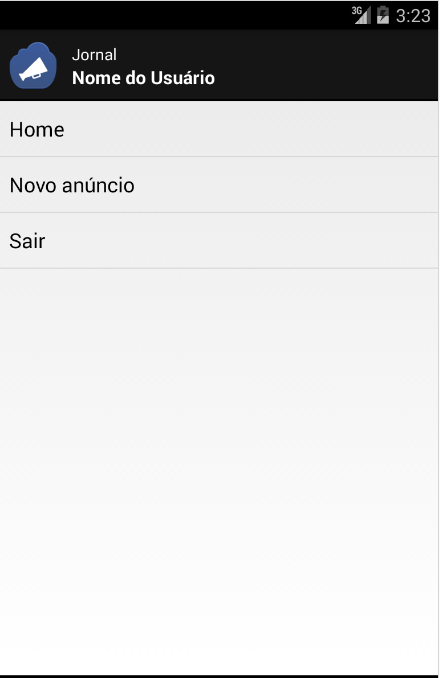
\includegraphics [scale=0.6]{imagens/android-menu.png}
		\fonte{AUTOR (2014)}\label{fig-android-menu}
	\end{center}
\end{figure}

A figura \ref{fig-android-novo-anuncio} apresenta a tela de cadastro de um novo anúncio, ela apresenta os campos de "Título" e "Texto", respectivos do anúncio e um menu com as opções "Salvar" e "Voltar". Ao selecionar a opção "Salvar" salva o aplicativo na base de dados e volta a tela de Menu e a opção "Voltar", apenas volta para a tela de Menu sem salvar o anúncio. \\ \\ \\ \\ \\ \\ \\ \\ \\ \\

\begin{figure}[h]
	\begin{center}
		\caption{
			\textbf{Tela de cadastro de anúncio}
		}\label{fig-android-novo-anuncio}
		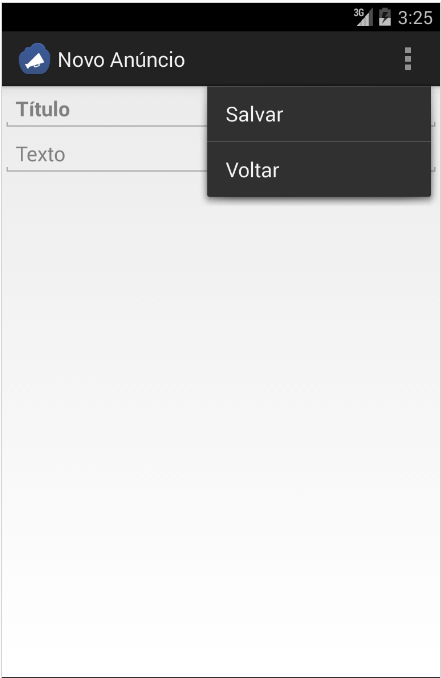
\includegraphics [scale=0.6]{imagens/android-novo-anuncio.png}
		\fonte{AUTOR (2014)}\label{fig-android-novo-anuncio}
	\end{center}
\end{figure}


\subsection{Aplicação Web}

Foi desenvolvido um protótipo de uma aplicação web que permite aos funcionários do veículo visualizar todos os anúncios cadastrados no banco de dados. Através de uma tela o usuário da aplicação pode ver listado todos os aplicativos e também visualizar detalhadamente cada anúncio listado.

A figura \ref{fig-anuncios-web} apresenta a tela com todos os anúncios cadastrados no banco de dados. Através do botão "Visualizar anúncio" é possível visualizar detalhadamente o anúncio da linha selecionada. \\ \\ \\ \\ \\ \\ \\ \\

\begin{figure}[h]
	\begin{center}
		\caption{
			\textbf{Tela visualização de todos os anúncios}
		}\label{fig-anuncios-web}
		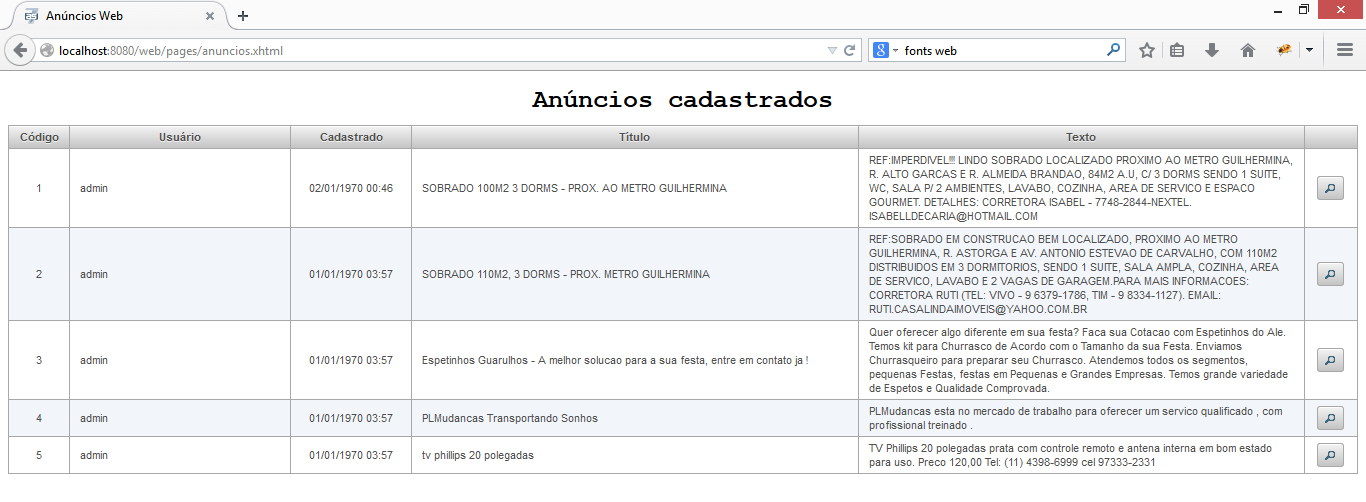
\includegraphics [scale=0.4]{imagens/anuncios-web.png}
		\fonte{AUTOR (2014)}\label{fig-anuncios-web}
	\end{center}
\end{figure}

A figura \ref{fig-anuncio-web} apresenta a tela com os detalhes do anúncio selecionado.

\begin{figure}[h]
	\begin{center}
		\caption{
			\textbf{Tela visualização de anúncio selecionado}
		}\label{fig-anuncio-web}
		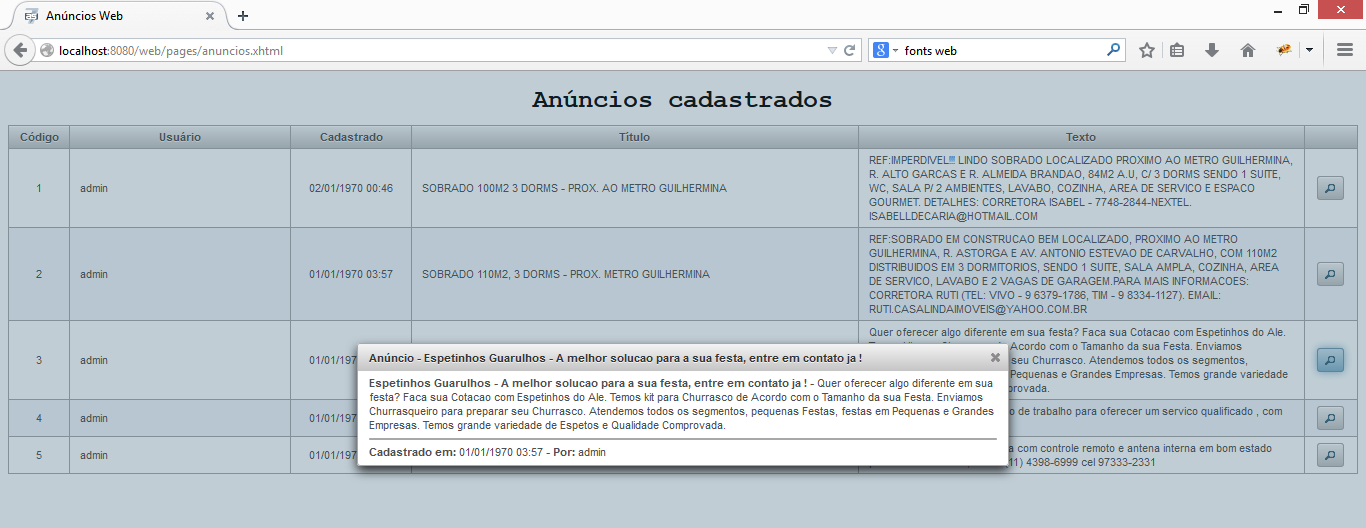
\includegraphics [scale=0.4]{imagens/anuncio-web.png}
		\fonte{AUTOR (2014)}\label{fig-anuncio-web}
	\end{center}
\end{figure}

% ---
% Conclusão
% ---
\chapter{CONCLUSÃO}

Este trabalho teve como propósito analisar e modelar o processo que envolve a captação de anúncios de uma empresa de mídia impressa utilizando BPM. A partir do modelo desenvolvido, realizar o aperfeiçoamento do mesmo, propor um novo modelo de processo e desenvolver um protótipo de aplicativo \textit{mobile} que contemplasse o modelo do processo de negócio proposto.

Todos os objetivos iniciais do trabalho foram concluídos com sucesso, o modelo de processo atual foi analisado e modelado com um diagrama de macroprocesso, partindo deste modelo, foi possível identificar melhorias a serem oferecias no processo, como resultado desta identificação,  foi proposto um novo modelo de processo de negócio através de outro diagrama de macroprocesso. Além do protótipo do aplicativo \textit{mobile}, foi possível também desenvolver um módulo \textit{web} extra, que agregou ao valor trabalho, trazendo maior visibilidade do objetivo do aplicativo de fornecer autonomia ao cliente.

Para alcançar os objetivos traçados no início do projeto e tornar o trabalho uma contribuição real, foi necessário muito esforço e aprendizado. O autor obteve conhecimento significante em diversas áreas, desde a área de foco do trabalho, a captação de anúncios de mídias impressas, passando pela modelagem de processos de negócio e BPM, até chegar no desenvolvimento de aplicativos \textit{mobile} utilizando Android e a criação e comunicação de \textit{webservices} com aplicativos Android e aplicações \textit{web}.

As maiores dificuldades encontradas pelo autor durante o desenvolvimento deste trabalho foram a sua inexperiência com modelagem de processos de negócios, o fato de não conhecer e ter que aprender sobre o desenvolvimento de aplicativos \textit{mobile} para a plataforma Android. Porém sua maior dificuldade foi pelo fato de ter saído da empresa de desenvolvimento de \textit{softwares} para veículos de comunicação onde trabalhava e ter ido para outra empresa de desenvolvimento de \textit{softwares}, onde perdeu o contato próximo que possuía com o processo de negócio.

Uma das principais contribuições do trabalho, tanto para a área do curso, quanto para as outras áreas de conhecimento, foi a modelagem e documentação de um processo de negócio que é conhecido apenas pelos que estão envolvidos no cotidiano de um veículo de mídia impressa, porém não possuí uma documentação.

Outra principal contribuição, foi mostrar como um \textit{software} pode ser envolvido nas etapas de um processo para melhorá-lo e torná-lo mais otimizado. Porém foi possível identificar que este envolvimento não é uma simples tarefa, são necessários estudos, análise e modelagem tanto do processo como do \textit{software} a ser inserido no mesmo.

Como consequência do desenvolvimento do aplicativo \textit{mobile}, também foi possível analisar e perceber o forte crescimento do mercado de dispositivos móveis e de seus aplicativos, mostrando uma forte tendência do desenvolvimento de \textit{software} para a área de dispositivos móveis.

Tendo em vista que o trabalho possui um conteúdo amplo e que não foi possível abordá-lo por completo neste trabalho, devido ao tempo disponível para o desenvolvimento do mesmo ser curto, sugere-se como melhorias e trabalhos futuros uma análise mais aprofundada para aplicativo \textit{mobile}; o seu desenvolvimento por completo, como por exemplo as funcionalidades de autenticação de usuário, edição de anúncios e um módulo para contemplar o pagamento dos anúncios; análise e o desenvolvimento do módulo \textit{web} para os funcionários e clientes do veículo.


% **************************************************

% ----------------------------------------------------------
% ELEMENTOS PÓS-TEXTUAIS
% ----------------------------------------------------------
% \postextual

% ----------------------------------------------------------
% Referências bibliográficas
% Arquivos que devem ser alterados
\bibliography{alterar/referencias}

% ----------------------------------------------------------
% Glossário
% ----------------------------------------------------------
%
% Consulte o manual da classe abntex2 para orientações sobre o glossário.
%
%\glossary

% ----------------------------------------------------------
% Apêndices
% ----------------------------------------------------------

% Informações que devem ser alteradas
% **************************************************
% ---
% Inicia os apêndices
% ---


% Etiqueta para auxiliar contagem do numero de paginas do texto e dos elementos pos-textuais
\label{nropaginas}

% **************************************************

%---------------------------------------------------------------------
% INDICE REMISSIVO
%---------------------------------------------------------------------
\printindex

\end{document}
